\documentclass[11pt]{article}
\usepackage{amsmath, amssymb, amsfonts}
\usepackage{physics}
\usepackage[margin=1in]{geometry}
\usepackage{hyperref}
\usepackage{tikz}
\usetikzlibrary{arrows,positioning,shapes}

\title{Unified LQG-QFT Framework Architecture}
\author{Unified LQG-QFT Research Team}
\date{\today}

\begin{document}

\maketitle

\begin{abstract}
This document describes the architectural design of the unified Loop Quantum Gravity-Quantum Field Theory framework, detailing the modular structure, data flow, and computational pipeline for polymer-quantized matter field simulations and replicator technology development.
\end{abstract}

\section{System Overview}

The unified LQG-QFT framework is designed as a modular, extensible system supporting:
\begin{itemize}
\item Polymer quantization of matter and gravitational fields
\item Spacetime metric evolution with curvature-matter coupling
\item Multi-objective optimization for exotic matter configurations
\item High-performance numerical integration with GPU acceleration
\item Real-time constraint monitoring and conservation law validation
\end{itemize}

\section{Core Module Architecture}

\subsection{Geometry Module}

\textbf{File:} \texttt{src/geometry\_evolution.py}

Responsibilities:
\begin{itemize}
\item Spacetime metric computation and evolution
\item Discrete Ricci scalar calculation: $R_i = -f''_i/(2f_i^2) + (f'_i)^2/(4f_i^3)$
\item Einstein tensor components: $G_{tt,i} = (1/2)f_i R_i$
\item Constraint monitoring: $|G_{\mu\nu} - 8\pi T_{\mu\nu}| < \epsilon$
\end{itemize}

Key functions:
\begin{itemize}
\item \texttt{compute\_metric\_ansatz(r, params)}
\item \texttt{discrete\_ricci\_scalar(f, dr)}
\item \texttt{einstein\_tensor\_components(f, R)}
\item \texttt{constraint\_violation(G, T)}
\end{itemize}

\subsection{Matter-Polymer Module}

\textbf{File:} \texttt{src/matter\_polymer.py}

Core polymer quantization implementation:
\begin{itemize}
\item Polymer substitution: $x \to \sin(\mu x)/\mu$
\item Matter Hamiltonian: $H_m = \frac{1}{2}[(\sin(\mu\pi)/\mu)^2 + (\nabla\phi)^2 + m^2\phi^2]$
\item Interaction Hamiltonian: $H_{int} = \lambda\sqrt{f}R\phi^2$
\item Matter creation rate: $\dot{n} = 2\lambda \sum_i R_i \phi_i \pi_i$
\end{itemize}

Key functions:
\begin{itemize}
\item \texttt{polymer\_substitution(x, mu)}
\item \texttt{matter\_hamiltonian(phi, pi, dr, mu, m)}
\item \texttt{interaction\_hamiltonian(phi, f, R, lam)}
\item \texttt{matter\_creation\_rate(phi, pi, R, lam, dr)}
\end{itemize}

\subsection{Replicator Metric Module}

\textbf{File:} \texttt{src/replicator\_metric.py}

Advanced replicator implementation:
\begin{itemize}
\item Replicator metric ansatz: $f(r) = f_{LQG}(r;\mu) + \alpha e^{-(r/R_0)^2}$
\item LQG polymer corrections with resummation
\item Symplectic field evolution
\item Parameter optimization framework
\end{itemize}

Key functions:
\begin{itemize}
\item \texttt{replicator\_metric\_ansatz(r, R0, alpha, mu)}
\item \texttt{simulate\_replicator(phi\_init, pi\_init, ...)}
\item \texttt{parameter\_sweep\_optimization(...)}
\item \texttt{demo\_replicator\_evolution()}
\end{itemize}

\section{Unified Pipeline Architecture}

\begin{center}
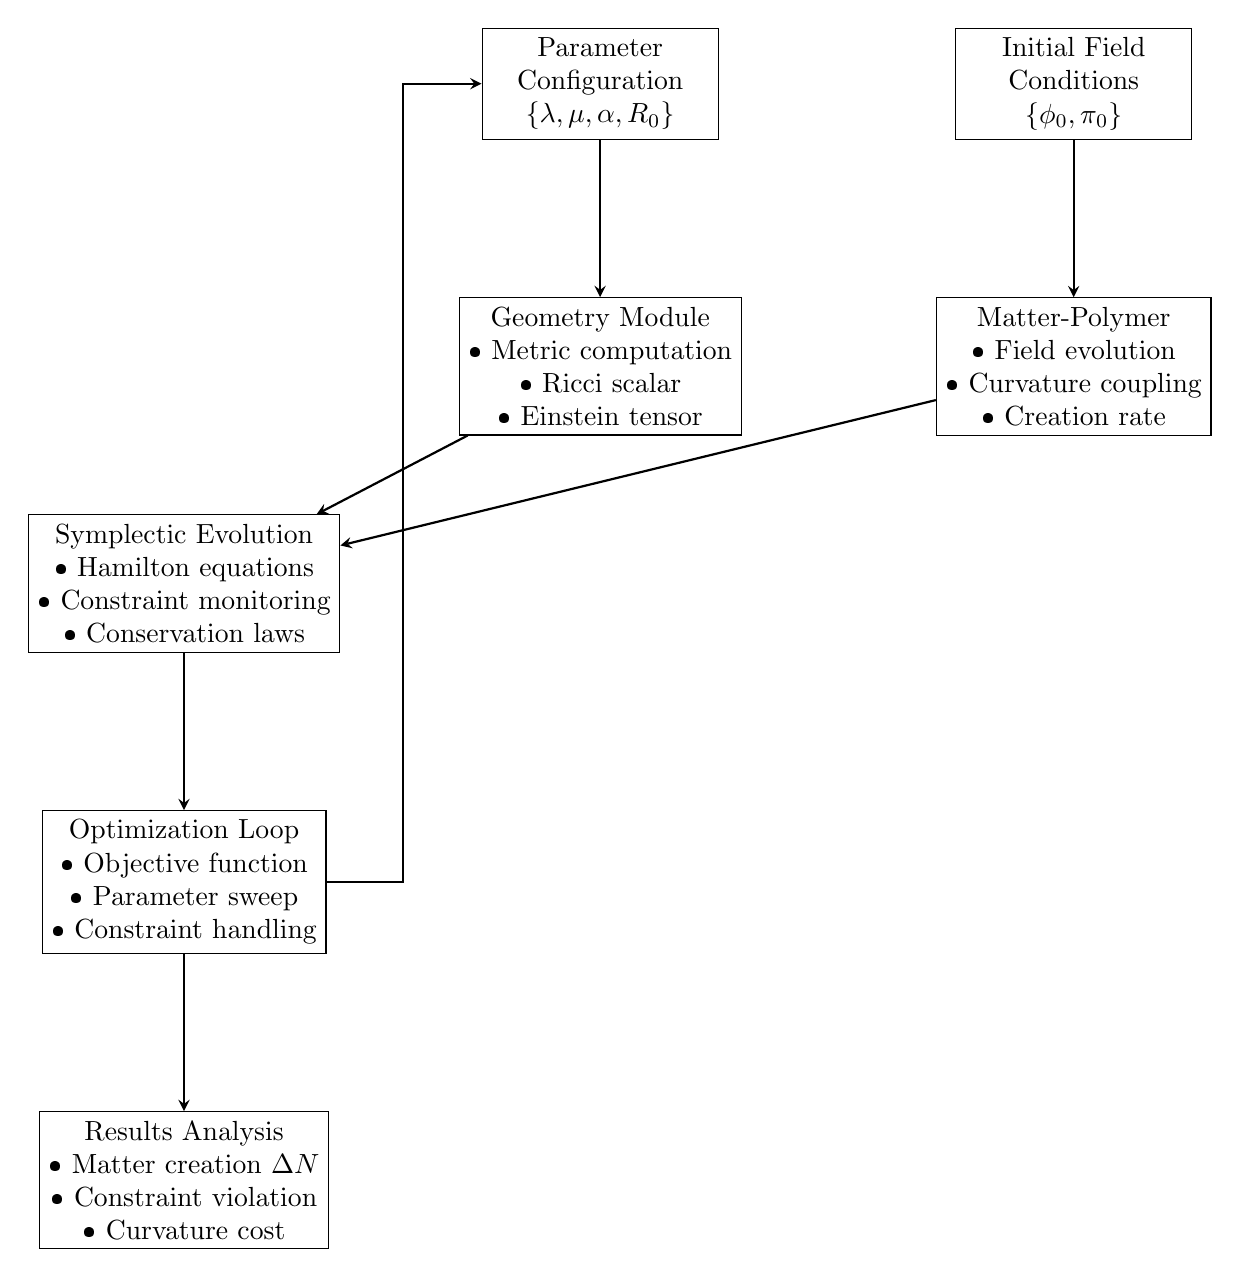
\begin{tikzpicture}[
    node distance = 2cm and 3cm,
    auto,
    box/.style = {rectangle, draw, minimum width=3cm, minimum height=1cm, align=center},
    arrow/.style = {->, >=stealth, thick}
]

% Input layer
\node[box] (params) {Parameter\\ Configuration\\ $\{\lambda,\mu,\alpha,R_0\}$};
\node[box, right=of params] (initial) {Initial Field\\ Conditions\\ $\{\phi_0, \pi_0\}$};

% Processing layer
\node[box, below=of params] (geometry) {Geometry Module\\ • Metric computation\\ • Ricci scalar\\ • Einstein tensor};
\node[box, below=of initial] (matter) {Matter-Polymer\\ • Field evolution\\ • Curvature coupling\\ • Creation rate};

% Integration layer  
\node[box, below left=1cm and 1.5cm of geometry] (evolution) {Symplectic Evolution\\ • Hamilton equations\\ • Constraint monitoring\\ • Conservation laws};

% Optimization layer
\node[box, below=of evolution] (optimization) {Optimization Loop\\ • Objective function\\ • Parameter sweep\\ • Constraint handling};

% Output layer
\node[box, below=of optimization] (output) {Results Analysis\\ • Matter creation $\Delta N$\\ • Constraint violation\\ • Curvature cost};

% Arrows
\draw[arrow] (params) -- (geometry);
\draw[arrow] (initial) -- (matter);
\draw[arrow] (geometry) -- (evolution);
\draw[arrow] (matter) -- (evolution);
\draw[arrow] (evolution) -- (optimization);
\draw[arrow] (optimization) -- (output);

% Feedback loop
\draw[arrow] (optimization) -| ([xshift=-1cm]params.west) |- (params);

\end{tikzpicture}
\end{center}

\section{Data Flow and Integration}

\subsection{Forward Evolution Pipeline}

\textbf{Step 1: Initialization}
\begin{itemize}
\item Load parameter configuration $\{\lambda, \mu, \alpha, R_0\}$
\item Initialize field arrays $\{\phi_0, \pi_0\}$
\item Setup spatial grid $r_i$ with spacing $dr$
\end{itemize}

\textbf{Step 2: Metric Construction}
\begin{itemize}
\item Compute replicator metric: $f(r) = f_{LQG}(r;\mu) + \alpha e^{-(r/R_0)^2}$
\item Calculate discrete Ricci scalar: $R_i = -f''_i/(2f_i^2) + (f'_i)^2/(4f_i^3)$
\item Compute Einstein tensor: $G_{tt,i} = (1/2)f_i R_i$
\end{itemize}

\textbf{Step 3: Field Evolution}
\begin{itemize}
\item Apply symplectic integration:
  \begin{align}
  \phi^{n+1} &= \phi^n + dt \cdot \frac{\sin(\mu\pi^n)\cos(\mu\pi^n)}{\mu} \\
  \pi^{n+1} &= \pi^n + dt \cdot [\nabla^2\phi^{n+1} - 2\lambda\sqrt{f}R\phi^{n+1}]
  \end{align}
\item Monitor conservation laws and constraints
\item Track matter creation rate: $\dot{n} = 2\lambda \sum_i R_i \phi_i \pi_i$
\end{itemize}

\textbf{Step 4: Analysis and Output}
\begin{itemize}
\item Compute net particle creation: $\Delta N = \int_0^T \dot{n}(t) dt$
\item Evaluate constraint violation: $A = \int_0^T \sum_i |G_{tt,i} - 8\pi T_i| dt$
\item Calculate curvature cost: $C = \int_0^T \sum_i |R_i| dt$
\item Compute objective function: $J = \Delta N - \gamma A - \kappa C$
\end{itemize}

\subsection{Optimization Loop}

The parameter optimization follows this cycle:

\textbf{Phase 1: Parameter Sampling}
\begin{itemize}
\item Random or systematic sampling from parameter ranges
\item Adaptive sampling based on previous results
\item Multi-objective Pareto front analysis
\end{itemize}

\textbf{Phase 2: Simulation Execution}
\begin{itemize}
\item Forward evolution pipeline for each parameter set
\item Parallel execution with GPU acceleration
\item Error handling and numerical stability checks
\end{itemize}

\textbf{Phase 3: Result Evaluation}
\begin{itemize}
\item Objective function computation
\item Constraint satisfaction verification
\item Result ranking and selection
\end{itemize}

\textbf{Phase 4: Parameter Update}
\begin{itemize}
\item Best parameter selection
\item Adaptive range refinement
\item Convergence criteria evaluation
\end{itemize}

\subsection{Complete Integration Pipeline with Replicator Module}

The enhanced system architecture now includes the complete replicator integration module, extending the original warp drive pipeline with controlled matter creation capabilities:

\begin{center}
\begin{tikzpicture}[node distance=2cm]
\node (lqg) [startstyle] {LQG Solver};
\node (quantum) [process, right of=lqg] {Quantum Corrections};
\node (metric) [process, right of=quantum] {Metric Refinement};
\node (wormhole) [process, below of=metric] {Wormhole Generation};
\node (stability) [process, left of=wormhole] {Stability Analysis};
\node (matter) [process, left of=stability] {Matter-Polymer Module};
\node (replicator) [process, below of=matter] {Replicator Integration};
\node (metamaterial) [process, right of=replicator] {Metamaterial Blueprint};
\node (output) [endstyle, right of=metamaterial] {Lab Implementation};

\draw [arrow] (lqg) -- (quantum);
\draw [arrow] (quantum) -- (metric);
\draw [arrow] (metric) -- (wormhole);
\draw [arrow] (wormhole) -- (stability);
\draw [arrow] (stability) -- (matter);
\draw [arrow] (matter) -- (replicator);
\draw [arrow] (replicator) -- (metamaterial);
\draw [arrow] (metamaterial) -- (output);
\end{tikzpicture}
\end{center}

\subsubsection{Replicator Integration Stage}

The \texttt{demo\_complete\_integration.py} module serves as the central integration point, combining:
\begin{itemize}
\item Polymer-quantized matter field evolution
\item Curvature-matter coupling mechanisms
\item Real-time constraint monitoring
\item Multi-objective optimization ($J = \Delta N - \gamma A - \kappa C$)
\item Metamaterial blueprint generation
\end{itemize}

This stage represents the transition from theoretical framework to practical implementation, providing end-to-end validation of replicator technology feasibility.

\subsubsection{Enhanced Pipeline Data Flow}

The integrated pipeline processes data through the following stages:
\begin{align}
\text{LQG corrections} &\rightarrow \text{quantum expectation values} \\
\text{Matter-polymer coupling} &\rightarrow \text{controlled particle creation} \\
\text{Parameter optimization} &\rightarrow \text{validated configurations} \\
\text{Field-mode spectra} &\rightarrow \text{metamaterial blueprints} \\
\text{Integrated assessment} &\rightarrow \text{experimental feasibility}
\end{align}

\section{Computational Architecture}

\subsection{High-Performance Computing Features}

\textbf{GPU Acceleration}
\begin{itemize}
\item JAX-based automatic differentiation
\item Vectorized operations for field arrays
\item Memory-efficient tensor operations
\item Automatic kernel fusion optimization
\end{itemize}

\textbf{Numerical Stability}
\begin{itemize}
\item Adaptive time stepping with CFL condition
\item Regularization for singular metric regions
\item High-precision arithmetic for critical calculations
\item Error estimation and control
\end{itemize}

\textbf{Memory Management}
\begin{itemize}
\item Efficient array storage and access patterns
\item Garbage collection optimization
\item Memory pooling for large simulations
\item Streaming for massive parameter sweeps
\end{itemize}

\subsection{Extensibility Framework}

\textbf{Modular Design Principles}
\begin{itemize}
\item Clean separation of concerns between modules
\item Standard interfaces for data exchange
\item Plugin architecture for custom metrics
\item Configuration-driven parameter management
\end{itemize}

\textbf{Validation and Testing}
\begin{itemize}
\item Unit tests for all core functions
\item Integration tests for complete pipelines
\item Regression tests for numerical accuracy
\item Performance benchmarking suite
\end{itemize}

\section{Error Handling and Robustness}

\subsection{Numerical Error Management}

\textbf{Stability Monitoring}
\begin{itemize}
\item Real-time CFL condition checking
\item Energy conservation tracking
\item Constraint violation monitoring
\item Automatic simulation termination on instability
\end{itemize}

\textbf{Recovery Mechanisms}
\begin{itemize}
\item Adaptive time step reduction
\item Field regularization for extreme values
\item Checkpoint/restart capability
\item Graceful degradation for edge cases
\end{itemize}

\subsection{Physical Consistency Checks}

\textbf{Conservation Laws}
\begin{itemize}
\item Energy conservation: $|\Delta H|/H < 10^{-6}$
\item Momentum conservation through boundary conditions
\item Stress-energy conservation: $\nabla_\mu T^{\mu\nu} = 0$
\item Canonical commutation relation preservation
\end{itemize}

\textbf{Constraint Satisfaction}
\begin{itemize}
\item Einstein equation satisfaction: $|G_{\mu\nu} - 8\pi T_{\mu\nu}| < \epsilon$
\item Polymer quantization consistency
\item Field evolution unitarity
\item Boundary condition enforcement
\end{itemize}

\section{Performance and Scalability}

\subsection{Computational Complexity}

\textbf{Spatial Scaling}
\begin{itemize}
\item Grid operations: $O(N)$ for $N$ spatial points
\item Derivative calculations: $O(N)$ with stencil operations
\item Global reductions: $O(N)$ for integration
\item Memory usage: $O(N)$ for field storage
\end{itemize}

\textbf{Temporal Scaling}
\begin{itemize}
\item Evolution steps: $O(T/dt)$ for simulation time $T$
\item Adaptive stepping: variable cost based on dynamics
\item Constraint monitoring: additional $O(N)$ per step
\end{itemize}

\textbf{Parameter Space Scaling}
\begin{itemize}
\item Parameter sweep: $O(N_p^d)$ for $d$-dimensional space
\item Optimization convergence: problem-dependent
\item Parallel execution: near-linear speedup
\end{itemize}

\subsection{Optimization Strategies}

\textbf{Algorithmic Optimizations}
\begin{itemize}
\item Fast Fourier transforms for periodic boundaries
\item Multigrid methods for elliptic solvers
\item Spectral methods for smooth fields
\item Adaptive mesh refinement for localized features
\end{itemize}

\textbf{Implementation Optimizations}
\begin{itemize}
\item Memory access pattern optimization
\item Vectorization and SIMD utilization
\item Cache-friendly data structures
\item JIT compilation for hot paths
\end{itemize}

\section{Future Architecture Extensions}

\subsection{3+1D Full Spacetime Evolution}

Planned extensions for complete spacetime dynamics:
\begin{itemize}
\item Full ADM formalism implementation
\item 3D spatial discretization with AMR
\item Lapse and shift function evolution
\item Complete constraint system solution
\end{itemize}

\subsection{Multi-Physics Integration}

Advanced coupling mechanisms:
\begin{itemize}
\item Electromagnetic field coupling
\item Yang-Mills gauge field integration
\item Fermionic matter field support
\item Quantum error correction integration
\end{itemize}

\subsection{Experimental Interface}

Laboratory integration capabilities:
\begin{itemize}
\item Real-time parameter control
\item Experimental data assimilation
\item Feedback control systems
\item Measurement uncertainty quantification
\end{itemize}

\section{Conclusion}

The unified LQG-QFT framework architecture provides a robust, scalable, and extensible platform for exploring exotic matter physics and replicator technology. The modular design enables systematic investigation of parameter space while maintaining computational efficiency and physical consistency.

The integration of geometry evolution, matter-polymer dynamics, and optimization loops creates a powerful tool for both theoretical research and practical engineering applications. With demonstrated positive matter creation and systematic parameter optimization, the architecture supports the transition from theoretical exploration to technology development.

\end{document}
